%%%%%%%%%%%%%%%%% your_thesis_eng.tex %%%%%%%%%%%%%%%%%
%
% This is the template file for ORM 2016 proceedings.
%
% Please, fill in following the directions below.
%
%%%%%%%%%%%%%%%%%%%%%%%%%%%%%%%%%%%%%%%%%%%%%%%%%%%%%%%

\newcommand{\No}{�}

\Title[%
% Insert here the acknowledgements of grants and/or any other
% information you wish to appear as a footnote, or leave this
% field blank.
The reported study was funded by RFBR according to the research project \No 16-01-00353a.%
]
{%
% Insert your title here
Multistage Bidding Model with Elements of Bargaining. Extension for a Countable State Space%
}
{%
% Insert the authors' names here
A.I.~Pyanykh%
}
{%
% Insert your institution here
Moscow State University%
}
{%
% Insert your city here
Moscow%
}
{%
% Insert your country here
Russia%
}

% Insert your thesis here.
% The entire submission should not exceed 3 pages if you plan a publication in conference proceedings.
%
% ATTENTION: Using 'thebibliography' environment is not allowed.
% Use 'references_eng' environment below to format the list of references.
% Please note that the latter environment does not provide automatic
% citation facilities. Cite manually using square brackets,
% e.g., [1], [2, 3], [4--6].
%
We consider a simplified model of a financial market with two players bidding for one unit of a risky asset (a share) for $n \leq \infty$ consecutive stages.
Player 1 (an insider) is informed about the liquidation price of the asset while Player 2 knows only its probability distribution.
At each stage players place integral bids.
The higher bid wins and a share is transacted to the winning player.
Each player aims to maximize the value of her final portfolio.

A model where the price takes only two values is considered in [1].
It is reduced to a zero-sum game with incomplete information on one side as in Aumann, Maschler [2].
It is shown that in this model uninformed Player 2 should use the history of Player 1's moves to update the posterior probabilities over the liquidation price of the asset via Bayes rule.
Thus Player 1's objective is to find such a strategy that allows him to strike a balance between taking advantage of his private information and concealing it from Player 2.

% Insert your figure, if needed.
% \begin{figure}[!h]
%   \centering
%   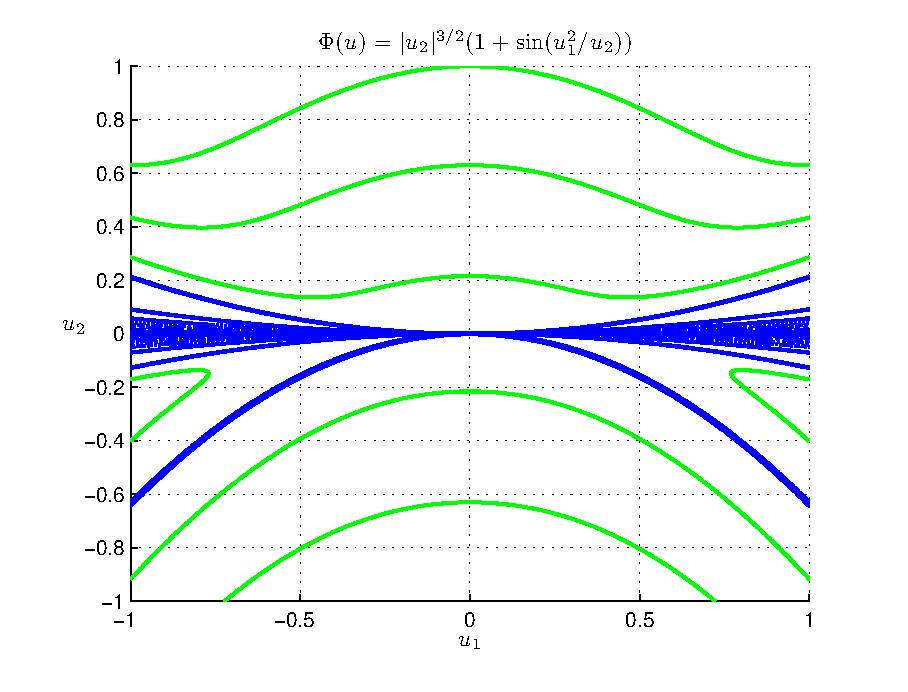
\includegraphics[width=0.7\maxpicturewidth]{your_figure.eps}
%   \center{Fig.~1. Your caption.}
% \end{figure}

\begin{references_eng}
% Insert your list of references here. The order of items in the list must
% agree with the order of their appearance in the text of your thesis.
% Use the '\url' command for citing url-s: e.g., \url{http://http://www.mathopt.org/}.

  \item % Reference No. 1
    Domansky~V. Repeated games with asymmetric information and random price fluctuations at finance markets // International Journal of Game Theory. 2007. V.~36, \No~2. P.~241--257.

  \item
    Aumann R.J., Maschler M.B. Repeated Games with Incomplete Information. Cambridge, Massachusetts: The MIT Press, 1995.

  \item % Reference No. 2
    Domansky~V.C., Kreps~V.L. Game Theoretic Bidding Model: Strategic Aspects of Price Formation at Stock Markets // The Journal of the New Economic Association. 2011. V.~11. P.~39--62.

  \item
    P'yanykh~A.I. A Multistage Exchange Trading Model with Asymmetric Information and Elements of Bargaining // Moscow University Computational Mathematics and Cybernetics. 2016. V.~40, \No~1. P.~35--40.
% ...

\end{references_eng}

%%%%%%%%%%%%%%%%%%%%%%%%%%%%%%%%%%%%%%%%%%%%%%%%%%%%%%%

%%% Local Variables:
%%% mode: latex
%%% TeX-master: "main"
%%% End:
